\chapter{Theory: Neural dynamics}
\label{chap:Neuron}
\index{Multicompartmental neuron model}
Extracellular potentials measured in neural tissue are primarily generated by the electrical activity of neurons, or more precisely, by neuronal transmembrane currents. To model extracellular potentials, we therefore first need to model neurons. Neural modeling is a core topic in computational neuroscience, and has been covered in several text books in much greater detail than we intend to include in this one (see e.g.,\cite**{johnston1994foundations,KockSegev1998,Koch1999,DeSchutter2000,Hille2001,Dayan2005,Izhikevich2007,Sterratt2011,Miller2018}) 


Frameworks exist for constructing neuronal models at various levels of detail and abstraction. In network models, it is common to represent each individual neuron as a single compartment, meaning that all its relevant variables, such as the membrane potential and transmembrane currents, are defined at a single point in space. Single compartment models, often called point-models\index{Point-model of neuron}, can give good predictions of neural firing rates, but do not generate extracellular potentials. The reason is current conservation: Currents travel in closed loops, and if a current enters a neuron at some at some location, the same amount of current must leave the neuron from other locations. Since point-models have no spatial extension, the currents must enter and leave on the same location, which in turn means that the sum of transmembrane currents is zero. Point models therefore do not generate any current sources that can generate extracellular potentials (\fref{fig:Neuron:point_vs_multi}A). Importantly, the fact that the membrane currents sum locally to zero does not mean that they do not affect the neuron. The current contains both an ionic and capacitive component, and the latter leads to dynamic changes in the membrane potential (see \fref{sec:Neuron:Cap}). 

\begin{figure}[!ht]
\begin{center}
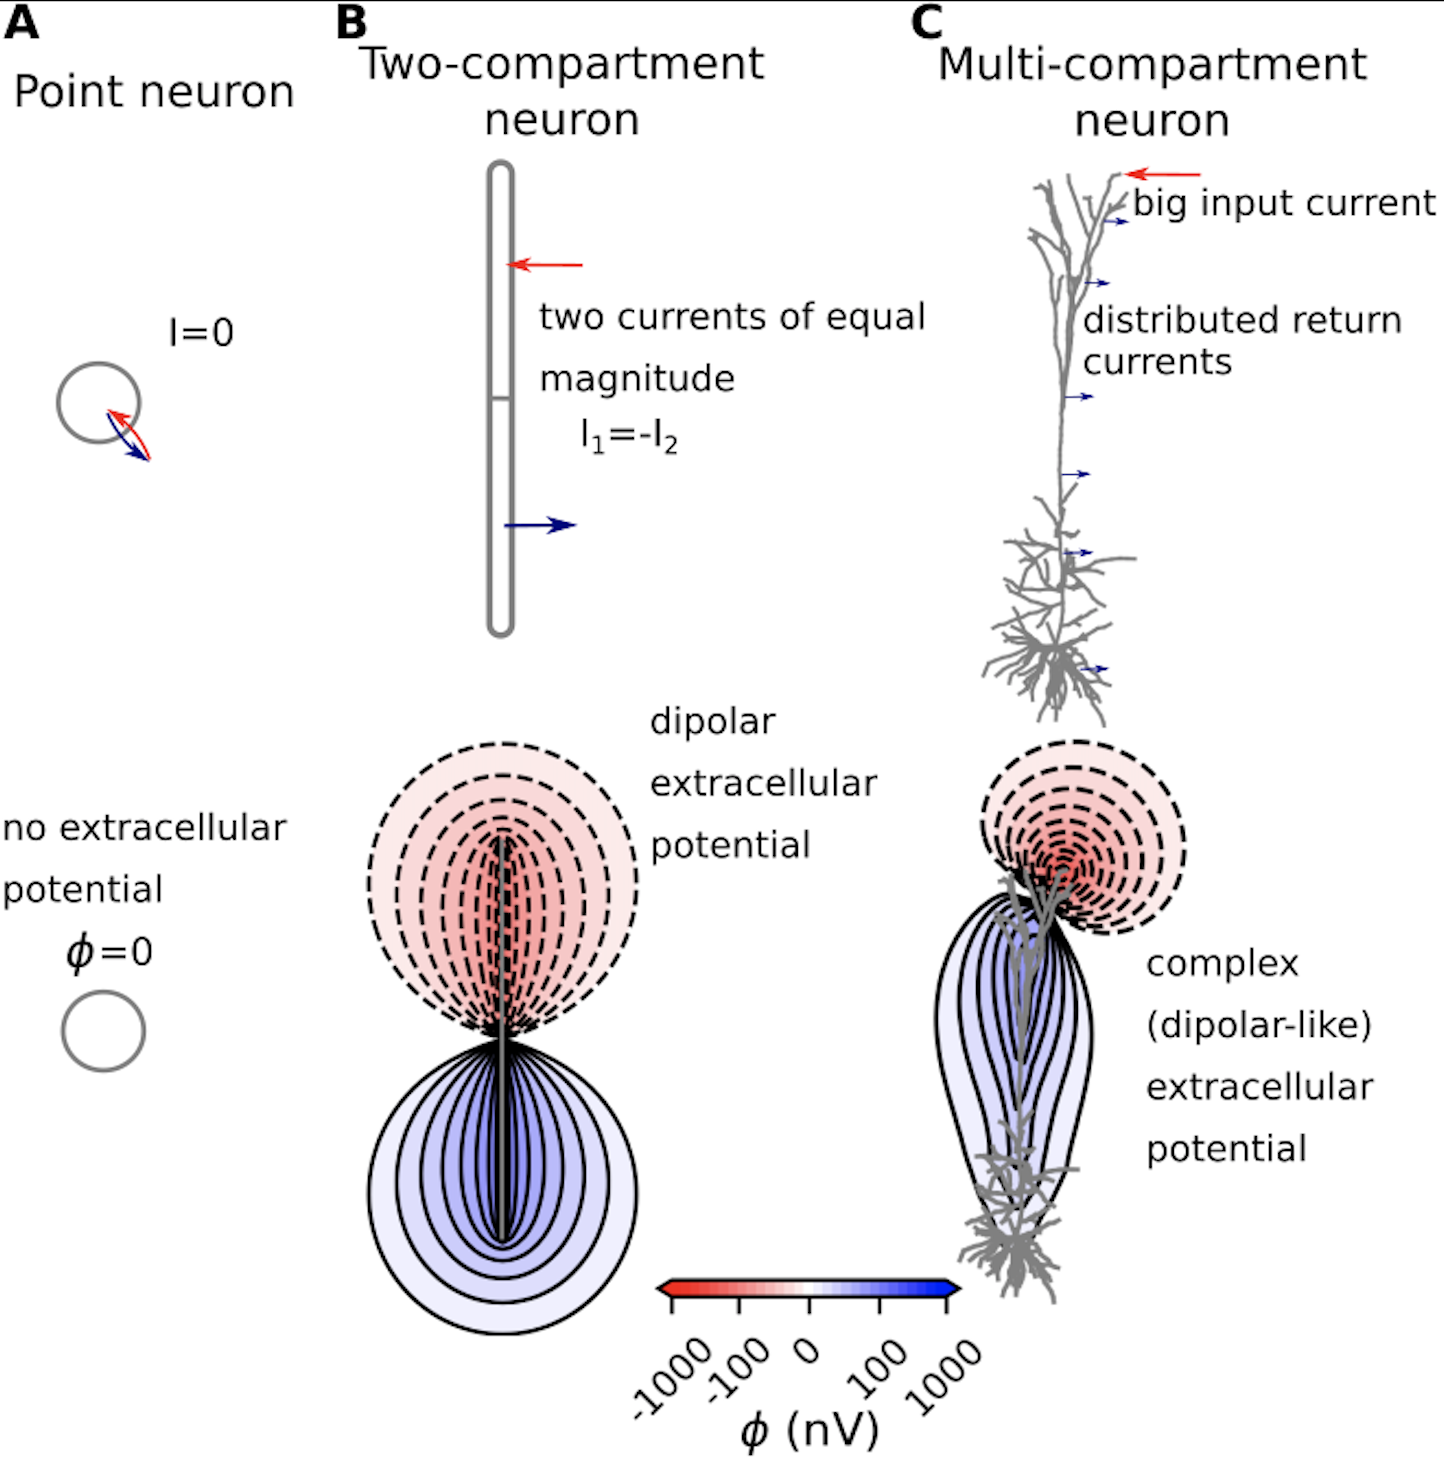
\includegraphics[width=0.6\textwidth]{Figures/Neuron/point_vs_multi}
\end{center}
\caption{\textbf{Fra bokkapittel.} }
\label{fig:Neuron:point_vs_multi}
\end{figure}

To account for the spatial extension of neurons, we need to use \textit{multicompartmental} (MC) neuron models. Also in MC models, the total sum of transmembrane currents must be zero. However, in MC models, currents do not have to enter and leave the neuron at the same location. MC models therefore give rise to a spatial distribution of currents entering (current sinks: current disappears from extracellular space) and leaving (current sources: currents appear in extracellular space) through the membrane (\fref{fig:Neuron:point_vs_multi}B-C).

The most common MC modeling framework combines a so-called \textit{Hodgkin-Huxley type} description of the neural membrane mechanisms (see e.g., \cite**{Hodgkin1952,KockSegev1998,Pospischil2008}) with cable theory to predict how signals propagate spatially in dendrites and axons (see, e.g., \cite**{Koch1999,rall2011}). This framework has become the gold standard for biophysically detailed neuronal simulations on the cellular and network level, and has been used for simulating the dynamics of large neuronal networks (see e.g., \cite**{traub2005,markram2015,billeh2020}.  We will here only present this standard framework, which we will refer to simply as the MC framework. 

An MC model is characterized by (i) its morphology, and (ii) its membrane mechanisms, and the key dynamical variable is the membrane potential ($V$). The morphology (i) of the real neuron (\fref{fig:Neuron:multicomp}A) is represented as a discretized set of compartments connected by resistors (\fref{fig:Neuron:multicomp}B). This structure houses two kinds of currents \fref{fig:Neuron:multicomp}C): (i) currents that run intracellularly between compartments (yellow arrows), and (ii) the transmembrane currents in each compartment (green arrows). Both currents depend (among other things) on the membrane potential in the various compartments, and together they determine how the membrane potential develops over time. 

\ghnote{Hva med denne versjonen?}

\begin{figure}[!ht]
\begin{center}
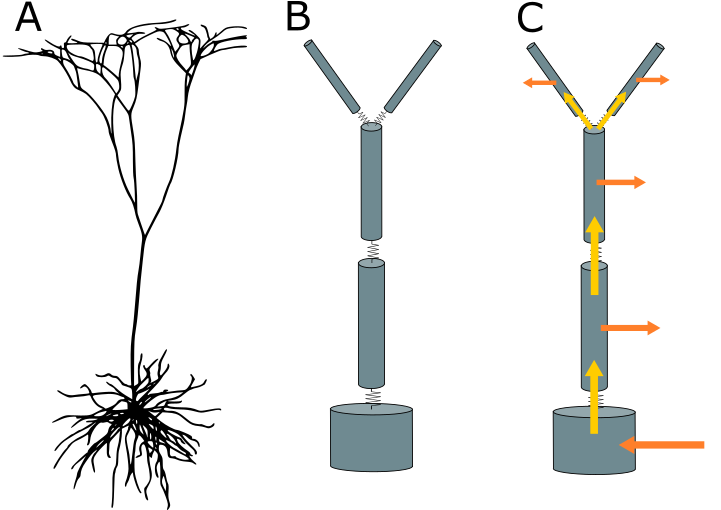
\includegraphics[width=0.6\textwidth]{Figures/Neuron/multicompartment.png}
\end{center}
\caption{\textbf{Multicompartmental modelling.}  (A) The neural morphology is (B) represented by a multicompartmental model, where the compartments are treated as cylinders connected by resistors. The example shows a crudely simplified model containing only five compartments, but detailed multicompartment models may include several hundreds of compartments, and can represent t he morphology in great detail. (C) Electric currents in the model can be separated into two groups: (i) transmembrane current in a compartment (green arrows), and (ii) intracellular currents between compartments (yellow arrows). 
}
\label{fig:Neuron:multicomp}
\end{figure}

Below, we first present a framework for modeling the transmembrane currents in a single compartment in \fref{sec:Neuron:membranecurrents}, and then go on to show how a number of such compartments can be connected together to a MC model in \fref{sec:Neuron:morphology}. Together, those two sections provide a theoretical framework for modeling neurons that should be sufficient for most practical applications. Readers that crave further biophysical insight into the ionic movements that mediate the transmembrane neural currents can get a brief introduction to this in \fref{sec:Neuron:Ions_and_reversals}. Finally, we end the chapter about neuronal modeling by briefly summarizing the main assumptions underlying the MC framework (\Fref{sec:Neuron:HHCassumptions}).


\section{\blue{Membrane currents}}
\label{sec:Neuron:membranecurrents}
\index{Hodgkin-Huxley type model}
Hodgkin-Huxley (HH) type models are called so because they describe the membrane mechanisms with a mathematical formalism similar to that used in celebrated model by \citeasnoun**{Hodgkin1952}. In HH-type models, the membrane typically includes three autonomous classes of transmembrane currents, normally represented as current densities (units \si{\ampere\per\square\metre}). These are (i) a capacitive current density ($i_{\mathrm{cap}}$), (ii) a leakage current density ($i_{\mathrm{L}}$), and (iii) a current density through active ion channels ($i_x$), of which there may be several different kinds ($x$ is an index). In addition, a neuron may receive stimuli, normally represented as total currents (units \si{\milli\ampere}). These can be either (iv) external current injections delivered by an experimentalist ($I_{\mathrm{ext}}$), or (v) synaptic input ($I_{\mathrm{syn}}$). In computer-modeling terminology, the membrane currents (i-iii) are often called distributed mechanisms, as they are membrane properties, and scale with the membrane area, while the stimuli (iv-v) are often called point-processes, as they are delivered on a singular point on the membrane. 

In the case where the neuron is modeled as a single compartment, the transmembrane currents into that compartment must sum to zero, so that:
\begin{equation}
i_{\mathrm{cap}}+ i_{\mathrm{L}} + \sum_x{i_x} +  \frac{I_{\mathrm{ext}} + I_{\mathrm{syn}}}{a_\text{c}} = 0,
\label{eq:Neuron:singlecomp_zerosum}
\end{equation}
where the point-currents must be divided by the compartment area $a_\text{c}$. Below, we define the various currents that go into this equation.

\subsection{\blue{Capacitive current}}
\label{sec:Neuron:Cap}
\index{Capacitive current}
The capacitive current density,
\begin{equation}
i_{\mathrm{cap}}= c_{\mathrm{m}} \frac{dV}{dt},
\label{eq:Neuron:HHcap}
\end{equation}
represents the charging up of the membrane to a potential $V$ due to a charge density accumulating on the outside and inside of the capacitive membrane. Here, $c_{\mathrm{m}}$ is the \textit{specific membrane capacitance} defined as capacitance per membrane area. In the original HH model, $c_{\mathrm{m}}$ had the value 1 \si{\micro \farad / \cm}$^2$, and this value seems to be representative for most neurons.  An illustration of how to interpret the capacitive current is given in \fref{fig:Neuron:capacitive_currents}. 

\begin{figure}[!ht]
\begin{center}
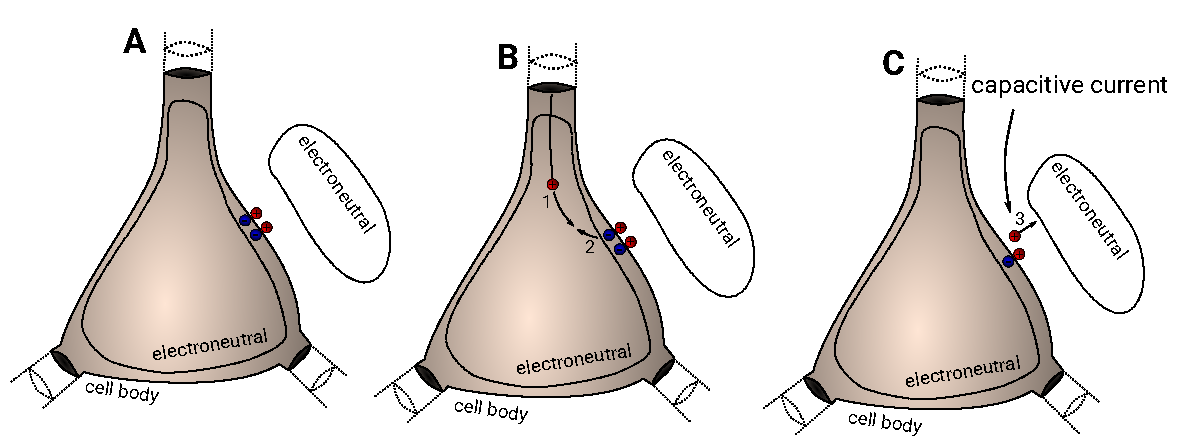
\includegraphics[width=1.0\textwidth]{Figures/Neuron/capacitive_currents.pdf}
\end{center}
\caption{\textbf{Capacitive currents ensure current conservation.} (\textbf{(A)}) The extracellular and intracellular bulk solutions are essentially electroneutral, and the only region where there is a nonzero charge density, is in thin Debye layers on either side of the capacitive membrane. The membrane separates a membrane charge density $\eta$ on one side from a membrane charge density $-\eta$ on the opposite side, giving rise to a membrane potential of $V = \eta/c_{\mathrm{m}}$. This charge separation process can be described in terms of a capacitive current: a transmembrane current that is not due to ions crossing the membrane, but due to ions piling up on either side of it.  An outward capacitive current could correspond to an anion leaving the membrane on the inside (\textbf{(B)}), which will coincide with a cation leaving the membrane on the outside (\textbf{(C)}). Thus, the capacitive current ensures current conservation. and gives rise to electrical ionic volume currents both in the intra- and extracellular space. \ghnote{Ny versjon av figurtekst. Ok?}
}
\label{fig:Neuron:capacitive_currents}
\end{figure}

If we insert \fref{eq:Neuron:HHcap} into \fref{eq:Neuron:singlecomp_zerosum}, we get:
\begin{equation}
c_{\mathrm{m}} \frac{dV}{dt} = - (i_{\mathrm{L}} + \sum_x{i_x} +  \frac{I_{\mathrm{ext}} + I_{\mathrm{syn}}}{a_\text{c}},
\label{eq:Neuron:singlecomp_capinserted}
\end{equation}
which gives us an intuitive understanding of neurodynamics: If the sum of ionic currents over the membrane (right hand side) is nonzero, it will lead to a charging up (left hand side) of the membrane.


\subsection{\blue{Leakage current}}
\label{sec:Neuron:leak}
\index{Leakage current}
The leakage current density is given by
\begin{equation}
i_{\mathrm{L}} = \bar{g}_{\mathrm{L}} (V - E_{\mathrm{L}}),
\label{eq:Neuron:HHleak}
\end{equation}
where $\bar{g}_{\mathrm{L}}$ is the leak conductance (the bar indicates that it's a constant). The factor $(V - E_{\mathrm{L}})$ (\si{\milli\volt}) is often called the \textit{driving force} and $E_{\mathrm{L}}$ the \textit{leak reversal potential}\index{Reversal potential}. The biophysical origin of the reversal potential is explained later (see \fref{sec:Neuron:Ions_and_reversals}). For now, we may simply think of $E_{\mathrm{L}}$ as the "target potential" that the leakage current will strive to drive the membrane potential towards. In reality, the leakage current is not a single current, but represents an orchestra of physiological processes that together will drive the membrane potential towards the value $E_{\mathrm{L}}$. 

Together, the capacitive current and the leakage current determine the passive properties of the membrane. If the neuron were to include only these two currents, it could be well modeled as an RC-circuit, and RC-neuron\index{RC-neuron} models are often used to simulate the subthreshold dynamics of neurons (\Fref{fig:Neuron:RC}). 

\begin{figure}[!ht]
\begin{center}
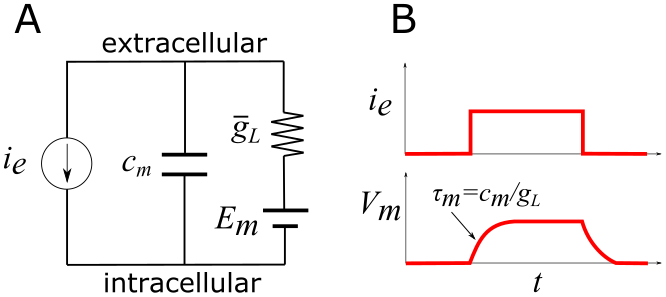
\includegraphics[width=0.8\textwidth]{Figures/Neuron/RCneuron.png}
\end{center}
\caption{\textbf{RC-neuron.}  A neuron model containing only a capacitive and a leakage current can be represented as an RC-circuit. To use standard MC modeling convention, we have expressed the various variables and parameters in units per membrane area: With a total membrane resistance $R = 1/(g_{\mathrm{L}} A)$, and capacitance $C = c_{\mathrm{m}}A$, we get that $RC = c_{\mathrm{m}}/g_{\mathrm{L}}$. In the illustration, the neuron is given an (electrode) injection $i_{\mathrm{e}}$ (A/cm$^2$) and responds by charging up the membrane. When the input is terminated, the membrane potential will return to the value $E_{\mathrm{L}}$. In the RC-model, $E_{\mathrm{L}}$ will be identical to the resting potential of the neuron, i.e., the potential that the membrane will settle on in the case where it does not receive any input. In models which include additional, active ion channels, these can in principle affect the resting potential, so that it may generally differ from $E_{\mathrm{L}}$.
}
\label{fig:Neuron:RC}
\end{figure}

We note that $\bar{g}_{\mathrm{L}}$ represents the \textit{specific conductance per unit area}, but we will simply refer to it as a \textit{conductance}. Its SI-base units are siemens per square meter (\si{\siemens\per\square\metre}), but in neuroscience applications it is common to use units millisiemens per square centimeter (\si{\milli\siemens\per\square\centi\metre}). 

\subsection{\blue{Active ion channels}}
\label{sec:Neuron:active}
\index{Ion channels! Voltage gated}
In addition to $i_{\mathrm{cap}}$ and $i_{\mathrm{L}}$, biophysical neuronal models include a number of active ion channels. These account for the fancy aspects of neurodynamics, and the main legacy of Hodgkin and Huxley was that they derived a mathematical model for describing the kinetics of these \cite**{Hodgkin1952}.

In the HH-type formalism, the current through an active ion channel type $x$ is modeled as:
\begin{equation}
i_x = \bar{g}_x m_x^{\alpha} h_x^{\beta}(V-E_x), 
\label{eq:Neuron:HHform}
\end{equation}
This current density $i_x$ does not represent the current through a single ion channel, but a large number of channels of the same type $x$. The constant, $\bar{g}_x$, denotes the conductance when all channels of type $x$ are fully open, while $E_x$ is the reversal potential for the ion species that travels through the channel type. In analogy with the leak reversal potential, we may think of $E_x$ as the target potential that the current through ion channel $x$ will strive to drive the membrane potential towards. The intrinsic membrane potential dynamics is thus due to the competition between various currents that all try to drive it towards their respective reversal potentials. 

If one prefers to think of neurons in terms of circuit diagrams, the active ion channels are simply added in parallel to the passive $i_{\mathrm{cap}}$ and $i_{\mathrm{L}}$ currents. As an example, the electric circuit representation of the HH model is depicted in \Fref{fig:Neuron:HH}.

\begin{figure}[!ht]
\begin{center}
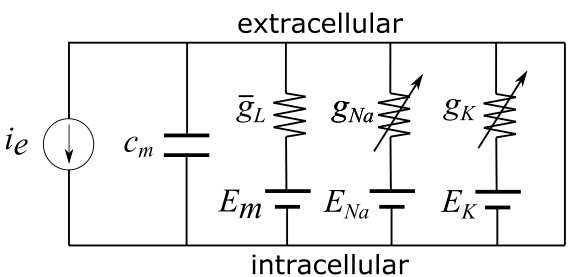
\includegraphics[width=0.8\textwidth]{Figures/Neuron/HHmodel.png}
\end{center}
\caption[]{\textbf{Active, single compartment neuron model.}  In addition to a capacitive and a leakage current, active neuron models contain a number of active ion channels. The example diagram shows the original Hodgkin-Huxley model, with an active Na$^+$ and an active K$^+$ channel. The arrows slicing the diagram conductances indicate that they are variables.}
\label{fig:Neuron:HH}
\end{figure}

Active ion channels differ from the passive leakage channel in that their total conductance, $\bar{g}_{x} m^{\alpha} h^{\beta}$, vary with time due to the so-called gating variables, in \fref{eq:Neuron:HHform} denoted $m$ and $h$\index{Gating variables}. These determine how the ion channels activate or deactivate (open or close), and $m$ and $h$ represent two different types of gates differing in terms of their opening/closing dynamics. The exponents $\alpha$ and $\beta$ represent the number of copies that a channel $x$ has of each type of gate. At the level of a single ion channel the values of $m$ and $h$ would interpret as the \textit{probability} that a given gate is in the open state. However, when we deal with summed currents through a large number of ion channels, the values of $m$ and $h$ interpret as the \textit{fraction} of the gates of the various types that are open. The values are thus numbers between 0 (all gates in the closed state) and 1 (all gates in the open state). The product $m^{\alpha} h^{\beta}$ thus interprets as the fractions of ion channels in which all gates are open so that currents can pass through. Consequently, the ion channel conductance is given by the product $\bar{g}_x m_x^{\alpha} h_x^{\beta}$.

For voltage-gated ion channels, the the dynamics of the gating variables can be described by kinetics equations on the form:
\begin{equation}
\frac{dx(V,t)}{dt} = \frac{x_{\infty}(V) - x}{\tau_x(V)},  \, \text{for } x \in \{m,h\}.
\label{eq:Neuron:HHgate}
\end{equation}
Here, the steady state activation $x_{\infty}(V)$, represents the fraction of gates that will end up in the open state if the cell is clamped at a given potential $V$ for sufficiently long time. However, the process of opening the gates takes some time, as accounted for by the activation time constant $\tau_x(V)$ (\si{\milli\second}). Both $x_{\infty}(V)$ and $\tau_x(V)$ are functions of the membrane potential, and these must be determined experimentally for each individual ion channel type. We do not go into the experimental challenges here, but will think of them as known functions. 

There are also many ion channels whose activation or inactivation do not depend on $V$, but on some other variable, such as the concentration of some ion species or ligand \cite**{Hille2001,Sterratt2011}. A common example are Ca$^{2+}$ gated ion channels, i.e., channels with gate opening controlled by the intracellular Ca$^{2+}$ concentration ($\mathrm{[Ca^{2+}]_i}$). There are also ion channels whose activation depend on more than one variable, such as e.g., ion channels whose activation depend on both $V$ and $\mathrm{[Ca^{2+}]_i}$. A HH-type formalism can in most cases be applied also to these kind of ion channels, provided that $x_{\infty}(V)$ and $\tau_x(V)$ in \fref{eq:Neuron:HHgate} can be replaced with experimentally determined functions of the relevant variables \cite**{Sterratt2011}.

To give an example of an active neuron model, the full set of equations for the HH model is summarized in Box \ref{box:Neuron:HH}. Compared to modern biophysically detailed neuron models, the original HH model is relatively simple in that it only contains two (voltage-gated) active ion channels, a Na$^+$ with three activation gates ($m^3$) and one inactivation gate ($h$), as well as a K$^+$ channel with four inactivation gates $n^4$. The two active ion channels are together responsible for action potential generation.  

\begin{floatingbox}[h]
\caption{Hodgkin-Huxley equations}

\begin{eqnarray*}
    c_{\mathrm{m}} \frac{dV}{dt} & =  & -\bar{g}_{\mathrm{L}}(V-E_{\mathrm{L}}) - \bar{g}_{\mathrm{Na}} m^3 h (V - E_{\mathrm{Na}}) - \bar{g}_{\mathrm{K}} n^4 (V - E_{\mathrm{K}}) \\
    \frac{dx(V,t)}{dt} & = & \frac{x_{\infty}(V) - x}{\tau_x(V)},  \, \text{for } x \in \{m,h,n\} \\ 
    x_{\infty}(V) &= & \frac{\alpha_x(V)}{\alpha_x(V) + \beta_x(V)}, \, \text{for } x \in \{m,h,n\} \\ %\hline
    \tau_x(V) & = & \frac{1}{\alpha_x(V) + \beta_x(V)}, \, \text{for } x \in \{m,h,n\} \\ %\hline
    \alpha_n &=& 0.01 \frac{V+55}{1-e^{-(V+55)/10}}  \\ %\hline
     \beta_n &=& 0.125 e^{-(V+65)/80}   \\ %\hline
     \alpha_m &=& \frac{0.1V+ 40}{1-e^{-(V+40)/10}}  \\   
     \beta_m &=& 4e^{-(V+65)/18}  \\ %\hline
    \alpha_h &=& 0.07e^{-(V+65)/20}  \\ %\hline
    \beta_h &=& \frac{1}{1+e^{-(V+35))/10}}   \\ %\hline
    c_\mathrm{m} &=& 1.0 \,\si{\micro\farad\per\square\centi\metre} \\ %\hline
    \bar{g}_{\mathrm{Na}} &=& 120 \,\si{\milli\siemens\per\square\centi\metre}\\ %\hline
    \bar{g}_{\mathrm{K}} &=& 36 \,\si{\milli\siemens\per\square\centi\metre} \\ %\hline
    \bar{g}_{\mathrm{L}} &=& 0.3 \,\si{\milli\siemens\per\square\centi\metre} \\ %\hline
    E_{\mathrm{Na}} &=& 50 \,\si{\milli\volt} \\ %\hline
    E_{\mathrm{K}} &=& -77  \,\si{\milli\volt} \\ %\hline
    E_{\mathrm{L}} &=& -54.4 \,\si{\milli\volt} \\ %\hline
\end{eqnarray*}
\\
Equations were taken from \citeasnoun**{Sterratt2011}. $V$ must be inserted with units \si{\milli\volt}
\label{box:Neuron:HH}
\end{floatingbox}

We note that the HH-type formalism for ion channels is a simplified approximation of the electrophysiological dynamics of ion channel currents and ion channel gating. Firstly, the currents described by \fref{eq:Neuron:HHform}, are sometimes called \textit{quasi-Ohmic}, as they are assumed to be proportional to the driving force $(V-E_k)$, when they in reality are nonlinear functions of both the ionic concentrations in the intra and extracellular space, and the membrane potential $V$ (for more on this, see \fref{sec:Neuron:GHK}). Secondly, since the HH-type formalism is based on deterministic equations, it cannot account for ion channel noise, which can stem from the stochastic gating at the single channel level. Thirdly, when channels open and close, movement of charges in channel proteins give rise to a tiny current called the \textit{gating current}, which is not included in the HH formalism. Fourthly, the relatively simple gating kinetics described by HH-type channels is not accurate for all ion channels, and more detailed ion channel models have been developed, based on a formalism more compatible with statistical physics and thermodynamics, or even more detailed, Markov-type formalism based on single-channel recordings. More comprehensive overviews of alternative ion channel models can be found in other textbooks (e.g., \cite**{Koch1999,Hille2001,Sterratt2011}).

Despite its limitations, the HH-form (\fref{eq:Neuron:HHform}) is generally deemed as sufficient for modeling neurodynamics on the cellular level, because it gives good predictions of the membrane currents. 

\ghnote{Tok bort "assumptions" fra sistekapittel, og satte dem inn i relevante kapitler. La til en flik om Gautes gating current.}

\subsection{\blue{Stimulus currents and synapses}}
\label{sec:Neuron:stim}
\index{Stimulus currents}
The stimulus current in \fref{eq:Neuron:singlecomp_zerosum} can represent any external stimulus that a neuron receives. Typically, it is either taken to represent an experimental electrode injection or a synaptic input. Below we include some typical examples of stimuli used in neuron simulations. 

\subsubsection{Current injections}
An electrode injection such as a step-current injection is modeled as:
\begin{equation}
I_\text{ext}(t)= 
\begin{cases}
    \text{constant}, & \text{for } t \in [t_\mathrm{start}, t_\mathrm{end}] \\
    0,              & \text{otherwise},
\end{cases}
\label{eq:Neuron:injected}
\end{equation}
Of course, one may chose the stimulus to be any function of time.


\subsubsection{Conductance-based synapses}
\index{Synapse}
\label{sec:Ch-Neuron:conductance-based-synapses}
A chemical synapse can be modeled more or less like an ion channel:
\begin{equation}
I_\text{syn}(t) = {G}_\text{syn}(t) \big(V(t)-E_\text{syn} \big), 
\label{eq:Neuron:chemicalsynapse}
\end{equation}
where $G_\text{syn}(t)$ is the synaptic conductance and $E_\text{syn}$ is the reversal potential of the synapse. The SI-base unit of a conductance is siemens (\si{\siemens}), but in neuroscience applications it is common to use units millisiemens (\si{\milli\siemens}) for $G_\text{syn}(t)$. We have denoted the synaptic conductance with a capitol $G$ to distinguish it from the specific conductances per unit membrane area ($g$) of ion channels.

The value of $E_\text{syn}$ determines whether the synapse is \textit{excitatory}, which means that it will tend to drive the  membrane potential of neuron toward the threshold for generating action potentials, or \textit{inhibitory}, which means that it will tend to drive the neuron away from the threshold for generating action potentials. Examples of excitatory synapses are AMPA and NMDA synapses, in which $E_\text{syn}$ ($\sim$ 0 \gex{--} 10 mV) is high above the neuronal resting potential. The most common inhibitory synapse is the GABA synapse, in which $E_\text{syn}$ ($\sim$ -70 mV) is close to the resting membrane potential of the neuron.

The synapse model described by \fref{eq:Neuron:chemicalsynapse} is called \textit{conductance based}, because the activation of the synapse is modeled as a transient change in the synaptic conductance. Unlike for ion channels, which are often voltage or calcium activated, the chemical synapse is activated by neurotransmitters received from a pre-synaptic cell. However, in MC type models, the transmitter-activation processes occurring in the synaptic cleft are normally not explicitly described. Instead, one normally uses a phenomenological synapse model, where the synaptic conductance $G_\text{syn}(t)$ is represented as a constant $\bar{G}_\text{syn}$ multiplied with a temporal kernel determining the opening and closing of a synapse set off at an activation time $t_s$:
\begin{equation}
I_\text{syn}(t) = \bar{G}_\text{syn} f(t) \big(V(t)-E_\text{syn} \big).
\label{eq:Neuron:chemicalsynapse}
\end{equation}
Typical choices for $f(t)$ are\index{Synapse models}: 
\begin{align}
&\text{(i) exponential decay:} \;\; f(t) = e^{-(t-t_\text{s})/\tau}\, \Theta(t-t_\text{s}) \\
&\text{(ii) $\alpha$-function:} \;\; f(t) =  \frac{t-t_\text{s}}{\tau} e^{-(t-t_\text{s})/\tau} \, \Theta(t-t_\text{s}) \\
&\text{(iii) $\beta$-function:} \;\; f(t) = \frac{\tau_1 \tau_2}{\tau_1-\tau_2} 
\Big( e^{-(t-t_\text{s})/\tau_1} - e^{-(t-t_\text{s})/\tau_2} \Big) \, \Theta(t-t_\text{s}) \\
& \text{(iv) NMDA-like:} \;\; f(t) = \frac{e^{-(t-t_\text{s})/\tau_1} - e^{-(t-t_\text{s})/\tau_2}} {1+\mu [\text{Mg}^{2+}] e^{-\gamma V} } \, \Theta(t-t_\text{s}),
\label{eq:Neuron:sf4}
\end{align}
where $\Theta(t)$ is the (Heaviside) unit step function: $\Theta(t \ge 0)=1$,  $\Theta(t< 0)=0$, and where parameters like $\gamma$,  $\tau$, $\tau_1$ and $\tau_2$ must be tuned to experimental data from the particular synapse type that one wants to model. The simple waveforms (i)--(iii) are typically used for AMPA  and GABA synapses, while the waveform (iv), is used for NMDA-synapses, where the conductance is influenced by membrane voltage and concentration of extracellular magnesium. 

The strength or efficacy of synaptic transmission may change over time through various processes that are often grouped together under the term "synaptic plasticity". Synaptic plasticity work as a mechanism for learning and memory formation in the brain. We will not go further into this topic here, but for more sophisticated synapse models, see e.g.,  \citeasnoun**{DeSchutter2000}.

\ghnote{Jeg sa ikke mer om saken enn dette. Kommentarer?}


\subsubsection{Current-based synapses}
\label{sec:Ch-Neuron:current-based-syn}
Unlike conductance-based synapses, which depend on the driving force, $V(t)-E_\text{syn}$ (\fref{eq:Neuron:chemicalsynapse}), 
current-based synapses are based on the approximation that the synaptic current is independent of the state ($V(t)$) of the neuron. The relationship between $\bar{G}_\mathrm{syn}$ and then becomes linear, so that the synapse can be modeled as:
\begin{equation}
I_\mathrm{syn}(t) = \overline{I}_\mathrm{syn} f(t).
\label{eq:Neuron:CurrentBasedSynapse}
\end{equation}
We can think of the current-based synapse as a conductance-based synapse where the driving force $V(t)-E_\text{syn}$ has been approximated by a constant (cf. \fref{eq:Neuron:chemicalsynapse}):
\begin{equation}
\bar{I}_\mathrm{syn}=\bar{G}_\mathrm{syn}(\langle V(t) \rangle_t -E_\mathrm{syn}),
\label{eq:Neuron:CurrentBasedAvg}
\end{equation}
where $\langle V(t) \rangle_t$ denotes the temporal average of the membrane potential. The temporal kernel
$f(t)$ can have the same exponential waveforms (i)-(iv) as for the conductance based synapses. Their relative conceptual and computational simplicity have made current-based synapses popular in large network simulations, and their linearity facilitates the derivation of analytical solutions \cite**{Richardson2004,Cavallari2014}. 

\subsubsection{Gap-junctions}
In addition to the chemical synapses, some neurons also form electrical synapses called \textit{gap junctions}. A gap junction is basically an electric coupling between a branch of one neuron (with membrane potential $V_1$) and a branch of another neuron (with membrane potential $V_2$). Essentially, we can think of this coupling as two neurons growing together into a continuous structure. The current through the gap junction is given by synaptic conductance multiplied with the voltage difference between the two coupled neural branches. 

\begin{equation}
I_\text{gap}=G_\text{gap} (V_{\mathrm{m}2}-V_{\mathrm{m}1}).
\label{eq:Neuron:gapjunction}
\end{equation}
This is conceptually similar to the currents between two compartments within a single multicompartment neuron (see \fref{sec:Neuron:morphology}).

%%%%%%%%%%%%%%%%%%%%%%%%%%
\section{\blue{Morphology}}
\label{sec:Neuron:morphology}
\index{Multicompartmental neuron model}
When we above introduced the various membrane currents, we mostly pictured the neuron as being a single compartment. In doing that, we implicitly assumed that the whole neuron was isopotential (same $V$ everywhere). However, in neurons with long and branchy dendrites, $V$ in the soma can be completely different from $V$ in the tip of a distal dendrite. If we want to account for the spatial aspect of neuronal signaling, we need to use multicompartmental (MC) models, where the neural morphology is represented as cylindrical compartments connected with resistors, and $V$ can be computed in each individual compartment (\Fref{fig:Neuron:multikompisen}A). 

\begin{figure}[!ht]
\begin{center}
\includegraphics[width=0.7\textwidth]{Figures/Neuron/multikompis.png}
\end{center}
\caption{\textbf{Multi-compartment model.} {\bf (A)} Representations of a neuronal morphology as a number of interconnected compartments. {\bf (B)} Subset of interconnected compartments. The currents involved in MC modeling include the sum of transmembrane currents ($I_{\mathrm{m},n}$) in a compartment $n$, and the intracellular currents running between 
compartments, $I_{n-1,n}$ (current from compartment $n-1$ to $n$), and $I_{n,n+1}$ (current from compartment $n$ to $n+1$).
}
\label{fig:Neuron:multikompisen}
\end{figure}

MC models rest on the assumption that neuronal morphology is well represented by a one-dimensional, branching cable. As such, MC type models neglect the radial components of intracellular currents (see e.g., \citeasnoun**{lindsay2004maxwell} for a critical study of this approximation). As a simple introduction to the formalism used in MC models, let us consider a subset of three connected cylindrical compartments which we number $n-1$, $n$ and $n+1$ (\Fref{fig:Neuron:multikompisen}B). For simplicity, we assume that the three cylinders have the same length ($L$) and diameter ($d$). The two categories of currents that run in this system are (i) the transmembrane currents that we introduced in the previous subsection, all of which we for now can group together into a total transmembrane current $I_{\mathrm{m},n}$, and (ii) the axial currents running between the cylindrical compartments ($I_{n-1,n}$ and $I_{n,n+1}$). The dynamics of this system is computed using Kirchhoff's current law, which demands that the sum of currents into a given compartment ($n$) should be zero:
\begin{equation}
I_{n-1,n} - I_{n,n+1} - I_{\mathrm{m},n} = 0.
\label{eq:Neuron:Kirch}
\end{equation}
We note that we here work with total currents (units \si{\ampere}), not current densities, so that $I_{\mathrm{m},n}$ is the sum of all current densities in the left hand side of \fref{eq:Neuron:singlecomp_zerosum} multiplied with the membrane area of compartment $n$. 

The axial current between two compartments is proportional to the voltage difference between the compartments, as determined by Ohm's law:
\begin{eqnarray}
I_{n-1,n} = \frac{V_{n-1}-V_n}{4 r_\text{a} L/(\pi d^2)}, \nonumber \\ 
I_{n,n+1} = \frac{V_{n}-V_{n+1}}{4 r_\text{a} L/(\pi d^2)}.
\label{eq:Neuron:axialcurrents}
\end{eqnarray}
Here, the denominators represent the axial resistance between two compartments, defined in terms of the axial resistivity $r_\text{a}$ (\si{\ohm\centi\metre}), a material property of the cytosol solution, the cross-section area, $\pi d^2/4$, and the segment length or travel distance, $L$.

The calculations become more complicated when the connected cylinders are of different length and diameter, and especially at branch points. However, the theory for computing the dynamics in branching structures with varying diameters is well established \cite**{Rall1977,Rall1989}, and designated software such as NEURON \cite**{Hines1997,Hines2009} automatizes the compartmentalization for the user once the neural morphology is specified. For the reminder of this chapter, we limit ourselves to consider the simplified, unbranched scenario (\Fref{fig:Neuron:multikompisen}B), as we deem this as sufficient for establishing an understanding of the essentials of MC modeling. 

We note that in \fref{eq:Neuron:axialcurrents}, $V_n$ is the \emph{intracellular} potential in compartment $n$. However, in most MC models, the intracellular potential is assumed to be identical to the membrane potential. This means that we assume that the extracellular potential $V_e = 0$. In turn, this amounts to assuming that the extracellular resistivity is zero, so that the extracellular space is isopotential and grounded. This may seem like a peculiar assumption to make in a book where the extracellular potential is the main topic. We comment further on this assumption and its consequences towards the end of this chapter. For now, we simply note that although the extracellular potential in reality is not zero, it is generally so much smaller than the intracellular potential that we can assume that it is zero without going too wrong when computing the neurodynamics. 
\ghnote{Er denne versjonen ok? Gikk ikke videre inn paa biologisk stoette for antakelsen $V_e = 0$.}



%%%%%%%%%%%%
\subsection{\blue{Active multicompartment models}}
\label{sec:Neuron:Active_multicomp}
To specify our MC neuron model further, we write out the total membrane current as:
\begin{equation}
I_{\mathrm{m},n} = I_{\mathrm{cap},n} + I_{\mathrm{ion},n} + I_{\mathrm{stim},n} = -\pi d L c_\text{m} \frac{dV_n}{dt} + \pi d L i_{\mathrm{ion},n} + I_{\mathrm{stim},n}
\label{eq:Neuron:Imemb}
\end{equation}
where $I_{\mathrm{ion},n}$ represents the total transmembrane ionic currents through leakage and active ion channels, and $I_{\mathrm{syn},n}$ can represent an electrode stimulus, a synaptic stimulus, or a combination of the two. In the last step, we expressed the capacitive and ionic currents (\si{\milli\ampere}) as current densities multiplied with the membrane area of the compartment ($a_\text{c} = \pi d L$) represented by the lateral sides of the cylinder, and we have inserted \fref{eq:Neuron:HHcap} for the capacitive current density. If we insert this into \fref{eq:Neuron:Kirch}, we get the fundamental equation for multicompartmental models:

\begin{equation}
c_\text{m} \frac{dV_n}{dt} = i_{\mathrm{ion},n} + \frac{d}{4r_\text{a}}\left(\frac{V_{n+1}-V_n}{L^2} - \frac{V_n-V_{n-1}}{L^2} \right) + \frac{I_{\mathrm{stim},n}}{\pi d L}.
\label{eq:Neuron:multimain}
\end{equation}
\Fref{eq:Neuron:multimain} assumes that a compartment $n$ has two neighbors ($n-1$ and $n+1$), which will not be true for the endpoint compartments of the simulated structure. To solve it, we must therefore select appropriate boundary conditions for these compartments. The most commonly used boundary condition is that of a sealed end, where $\frac{\partial V_n}{\partial x} = 0$ for $n$ at the endpoints, that no axial current leaves there.  This is for example the default boundary condition in the NEURON simulator. 

%%%%%%%%%%%%%%%%%
\subsection{\blue{Passive multicompartment models}}
\label{sec:Neuron:Passive_multicomp}
\index{Multicompartmental neuron model}
The neural response to small perturbations from the resting potential often has a close to linear relationship between the membrane potential and membrane currents \cite**{mauro1970,koch1984,ness2016}.\ghnote{Ha med disse refs eller ikke? Disse arbeidene driver jo med en linearisering og bruker ikke den enkle formen vi drar til med nedenfor. Samtidig gir de jo et argument for lineariteten vi postulerer.} When modeling subthreshold neural dynamics, a common simplification is therefore to assume that ionic membrane current density has the linear form,
\begin{equation}
i_{\mathrm{ion},n} = g_\text{m}(V_n - E_m),
\label{eq:Neuron:mleak}
\end{equation}
where $E_\text{m}$ is the membrane resting potential, and $g_\text{m}$ the specific membrane conductance. This is essentially the same as the passive leakage current density defined earlier (\fref{eq:Neuron:HHleak}), but with $g_\text{L}$ and $E_\text{L}$ replaced with $g_\text{m}$ and $E_\text{m}$, respectively. We may think of \fref{eq:Neuron:mleak} as comprising the leakage current as well as contributions from active currents that are linear (passive-like) and partly open near the resting potential. In simplified neuron models called \textit{integrate-and-fire} neurons, such a linear relationship between membrane currents and membrane potential is assumed to hold all the way up to the action-potential-firing threshold \cite**{Sterratt2011}. 

Models that approximate the transmembrane ionic current density with \fref{eq:Neuron:mleak} are often called passive. In passive models it is customary to replace the specific membrane conductance $g_\text{m}$ with the specific membrane resistance $r_\text{m} = 1/g_\text{m}$ (\si{\ohm\square\centi\metre}). For MC models, the passive version of 
\fref{eq:Neuron:multimain} then becomes:
\begin{equation}
c_\text{m} \frac{dV_n}{dt} = \frac{E_\text{m}-V_n}{r_\text{m}} + \frac{d}{4r_\text{a}}\left(\frac{V_{n+1}-V_n}{L^2} - \frac{V_n-V_{n-1}}{L^2} \right) + \frac{I_\text{stim}}{\pi d L}
\label{eq:Neuron:multipassive}
\end{equation}

Passive MC models (\fref{eq:Neuron:multipassive}) are often used as an approximation for signaling in neural dendrites, which tend to have a lower density of active mechanisms compared to the soma and axon. Sometimes, the passive approximation is used for all compartments in the MC model, for example to simulate responses to subthreshold synaptic input. 

An illustration of passive signal propagation is shown in \fref{fig:Neuron:Semiinf}A, which shows the membrane potentials at selected positions along a 1000~\si{\micro\metre} long stick-neuron responding to a stimulus resembling a synaptic input in one end. We see that the peak response comes faster in proximal than in distal locations, and that the peak response decays with distance from the synapse. We also see that potential at all points along the stick become level a few milliseconds after the stimulus was delivered, after which $V$ decays gradually towards the resting potential. These simulations on a passive model give a qualitative idea on how signals spread in dendrites. As we shall see below, the passive model is also useful in that it allows us to derive some analytical results for signal propagation in neural dendrites.

\begin{figure}[!ht]
\begin{center}
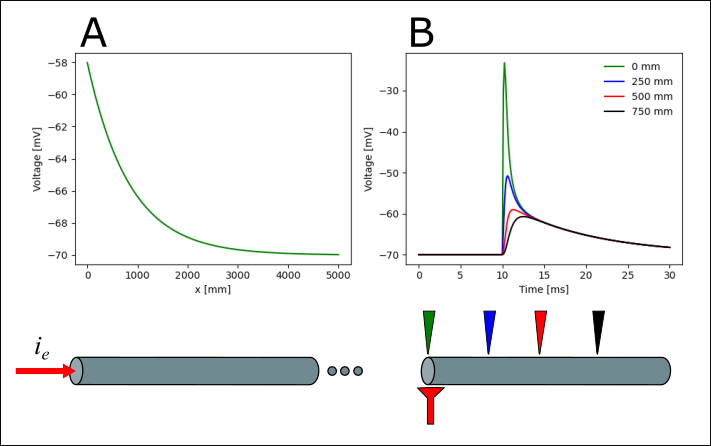
\includegraphics[width=0.7\textwidth]{Figures/Neuron/Cablesims.png}
\end{center}
\caption{\textbf{Stick-neuron responding to transient and constant inputs received in one end.} (A) Finite cable of length $L = 1 \, \si{\milli\metre}$ simulated numerically as 100 compartments, and stimulated with an alpha-synapse in the first compartment ($0<x<10 \, \si{\micro\metre}$). Transient responses shown at different distances from the synapse. The peak response decreases with distance from the synapse, and the time to reach the peak increases with distance from the synapse.
(A) Analytical steady-state solution for semi-infinite cable receiving a constant input $I_\text{stim} = 0.1 \, \si{\nano\ampere}$ in a sealed end at $x=0$. The membrane potential decays exponentially with distance from the stimulus site.  (A-B) Parameter choices: $c_\text{m}=1\, \si{\micro\farad\per\square\centi\metre}$, $d = 1\, \si{\micro\metre}$, $r_\text{a}=35.4\, \si{\ohm\centi\metre}$, $r_\text{m} = 10 \, \si{\kilo\ohm\square\centi\metre}$, which gives a length constant $\lambda = 840\, \si{\micro\metre}$.}
\label{fig:Neuron:Semiinf}
\end{figure}


%%%%%%%%%%%%%%%%%%%%
\subsection{\blue{Cable equation}}
\label{sec:Neuron:cableeq}
\index{Cable equation}
If we in \fref{eq:Neuron:multipassive} let $L \rightarrow \delta x$, and take the limit $\delta x \rightarrow 0$, we can derive the cable equation (see e.g., \cite**{Sterratt2011}): 

\begin{equation}
c_\text{m} \frac{\partial V}{\partial t} = \frac{E_\text{m}-V}{r_\text{m}} +  \frac{d}{4 r_\text{a}}  \frac{\partial^2 V}{\partial x^2}  + \frac{\mathcal{I}_{\mathrm{stim}}}{\pi d},
\label{eq:Neuron:cable}
\end{equation}
where we have introduced the stimulus current per unit length,
\begin{equation}
\mathcal{I}_{\mathrm{stim}}(x,t) = \lim_{\delta x \to 0} I_{\mathrm{stim}}(x,t)/\delta x \,\; (\si{\milli\ampere\per\centi\metre}). 
\label{eq:Neuron:CurrentPerUnitLength}
\end{equation}
To improve our analytical understanding of dendritic signaling, it is useful to reformulate the cable equation to:
\begin{equation}
\tau_\text{m} \frac{\partial V}{\partial t} = E_\text{m}-V +   \lambda^2  \frac{\partial^2 V}{\partial x^2}  + \frac{r_\text{m} \mathcal{I}_{\mathrm{stim}} }{\pi d},
\label{eq:Neuron:cable2}
\end{equation}
where we have multiplied all terms with $r_\text{m}$ and introduced the length constant \index{Length constant},
\begin{equation}
\lambda = \sqrt{\frac{d r_\text{m}}{4 r_\text{a}}} \,\; (\si{\centi\metre}), 
\label{eq:Neuron:lengthconst}
\end{equation}
and the time constant\index{Membrane time constant}, 
\begin{equation}
\tau_\text{m} \equiv r_\text{m} c_\text{m}  \,\; (\si{\milli\second}).
\label{eq:Neuron:timeconst}
\end{equation}
Here, $\tau_\text{m}$ is typical time scale (dimensionless time: $t/\tau$), while $\lambda$  is typical length scale  (dimensionless length: $x/\lambda$) for signals in the cable. If a certain point along the cable is perturbed, so that the potential is shifted from rest to a given value $V$, $\tau_\text{m}$ will determine how fast the local potential falls back towards rest, while $\lambda$ will tell us how far the local perturbation will spread along the cable. 

The cable equation is a continuous version of \fref{eq:Neuron:multipassive}. Whereas MC models generally must be solved numerically, the cable equation allows the spatiotemporal evolution of the membrane potential to be solved analytically for some idealized scenarios. Below, we consider a couple of scenarios that will  make the interpretation of $\tau_\text{m}$ and $\lambda$ clearer. 


%%%%%%%%%%%%%%%%%%%%
\subsection{\blue{Steady state solution of the cable equation}}
\label{sec:Neuron:cableSS}
Let us find the steady state solution for a semi-infinite cable, receiving a constant current injection at a sealed end in $x=0$ (\Fref{fig:Neuron:Semiinf}B). Since only the end-point receives the stimulus, we may attack this problem by solving \fref{eq:Neuron:cable2} for all other points $x>0$, and then incorporate the effects of the stimulus current later as a boundary condition. 

At steady-state, $\partial V/\partial t = 0$, and \fref{eq:Neuron:cable2} becomes:
\begin{equation}
0 = E_\text{m}-V +  \lambda^2 \frac{\partial^2 V}{\partial x^2},
\label{eq:Neuron:semiinf}
\end{equation}
at all points along the cable, except $x=0$. If we introduce the new variable $\Delta{V}=V-E_\text{m}$, \fref{eq:Neuron:semiinf} simplifies to:
\begin{equation}
\frac{d^2 \Delta{V}}{d x^2} -  \frac{1}{\lambda^2} \Delta{V}=0, 
\label{eq:Neuron:semiinf2}
\end{equation}
which has the solution:
\begin{equation}
\Delta{V}(x) = \Delta{V}(0) e^{-x/\lambda}, 
\label{eq:Neuron:semiinf3}
\end{equation}
or, 
\begin{equation}
V(x) = E_\text{m} + \big( V(0)-E_\text{m} \big) e^{-x/\lambda}.
\label{eq:Neuron:semiinf4}
\end{equation}
We note that the general-solution to \fref{eq:Neuron:semiinf2} also has a term containing $e^{+x/\lambda}$, but this term diverges when $x \rightarrow \infty$ and was excluded on the count of being unphysical.

To obtain the final solution of the problem, we need to specify the boundary value $V(0)$, which will depend on the stimulus current. Since the stimulus is injected in a singular point ($x=0$), we go back to expressing in terms of a total current, $I_\text{stim}$ (and not as a current per unit length $\mathcal{I}_\text{stim}$). We can introduce it through a boundary condition demanding that the injected current must be identical to the axial current in the cable at $x=0$:
\begin{equation}
I_\text{stim} = - \frac{\pi d^2}{4}\frac{1}{r_\text{a}} \frac{\partial V}{\partial x}   \Big|_{x=0}.
\end{equation}
If we insert for $\partial V/\partial x$ (calculated from \fref{eq:Neuron:semiinf4}), and insert \fref{eq:Neuron:lengthconst} for $\lambda$, we can derive the following expression for $V(0)$:
\begin{equation}
V(0) = E_\text{m} + R_{\infty}I_\text{stim}, 
\label{eq:Neuron:firstRinf}
\end{equation}
where we have defined:
\begin{equation}
R_{\infty} = \sqrt{\frac{4 r_\text{m} r_\text{a}}{\pi^2 d^3}}.
\label{eq:Neuron:Rinf}
\end{equation}
If we now insert \fref{eq:Neuron:firstRinf} into \fref{eq:Neuron:semiinf4}, we obtain our final solution:
\begin{equation}
V(x) = E_\text{m} +R_{\infty}I_\text{stim}  e^{-x/\lambda}.
\label{eq:Neuron:semiinf5}
\end{equation}

The steady state solution to the semi-infinite cable (plotted in \Fref{fig:Neuron:Semiinf}B) is useful as it gives us analytical insight into signals spreading in e.g., passive dendrites. Some insights that can be derived from it is:

\begin{itemize}
\item It follows from \fref{eq:Neuron:firstRinf} that $R_{\infty} = (E_\text{m}-V(0))/I_\text{stim}$ interprets as the steady-state input resistance of the semi-infinite cable. \Fref{eq:Neuron:Rinf} thus shows that the input resistance is proportional to $1/d^{3/2}$, i.e., the input resistance is higher the thinner the dendrite. 

\item \Fref{eq:Neuron:semiinf4} shows that in steady-state, the amplitude will decay exponentially from the injection site and outwards, and will be reduced by a factor $1/e$ over the length $\lambda$. If we insert some typical values into \fref{eq:Neuron:lengthconst}, like a dendritic diameter of $d=1 \, \si{\micro\metre}$, a membrane resistance of $R_\text{m}=10 \,
\si{\kilo\ohm\square\centi\metre}$, and an axial resistivity $R_\text{a}=35.4\, \si{\ohm\centi\metre}$ we get a length constant of $\lambda = 840\, \si{\micro\metre}$. Dendrites with lengths in this order will thus only be moderately affected by the membrane potential in the soma. \ghnote{Vudere andre params her og i fig over. Disse var fra Fig 2.17 i Sterratt.}

\item According to \fref{eq:Neuron:lengthconst}, $\lambda \propto \sqrt{d}$, meaning that signals will spread further the thicker the dendrite.

\item According to \fref{eq:Neuron:lengthconst}, $\lambda \propto \sqrt{R_\text{m}/R_\text{a}}$ meaning that the signal is facilitated by having a large membrane resistance compared to axial resistance. 
\end{itemize}


%\subsection{\blue{GH: Temporal solutions of cable equation}}
%\label{sec:Neuron:cabletemp}
%\tvnnote{Bruker vi dette noe sted?}
%In \fref{fig:Neuron:Semiinf}A we simulated numerically the response of a cylindrical neuron to a  synaptic input in one end. It is possible to show analytically that the passive decay of $V$ following the input-induced peaks can be expressed as a sum of exponentials \cite**{rall1969}:
%\begin{equation}
%V(x,t) = C_0(x) e^{-t/\tau_0} + C_1(x) e^{-t/\tau_1} + C_2(x) e^{-t/\tau_2} + \ldots, 
%\label{eq:Neuron:cabletemporal}
%\end{equation}
%where the coefficients $C_n(x)$ depend on the distance along the cable, while $\tau_0 = \tau_\text{m} = R_\text{m} c_\text{m}$ is the \emph{membrane time constant} (\fref{eq:Neuron:timeconst}), and the other time constants have successively smaller values ($\tau_0 > \tau_1 > \tau_2 > \ldots$). We will not here present these analytical results in any further detail, but note that the final decay phase, i.e., when $V$ at all locations have coincided, takes place at the slower time scale of the membrane time constant, $\tau_\text{m}$ which in the simulation in \Fref{fig:Neuron:Semiinf}A  was 10 \si{\milli\second} ($R_\text{m}=10\,\si{\kilo\ohm\square\centi\metre}$, and $c_\text{m}=1\, \si{\micro\farad\per\square\centi\metre}$). 


\subsection{\blue{Frequency dependence of the length constant}}
\label{sec:Neuron:cablefreq}
As we just saw, the length constant $\lambda$ (\fref{eq:Neuron:lengthconst}) is the length over which the potential falls to a fraction $1/e$ of its boundary value when the finite end of a semi-infinite cable is fixed at a constant potential, or, equivalently, if the end of a semi-infinite cable receives a constant direct-current (DC) input. Therefore, $\lambda$ is often referred to as the DC length constant. 

It is possible to derive a corresponding length constant for AC input to a semi-infinite cable \cite**{johnston1994foundations}: 
\begin{equation}
\lambda_{AC} = \lambda \sqrt{ \frac{2}{1+\sqrt{(\omega \tau)^2 + 1}} }.
\label{eq:Neuron:AClambda}
\end{equation}
Here $\tau_\text{m}$ is still the membrane time constant (\fref{eq:Neuron:timeconst}), $\lambda$ is still the DC length constant (\fref{eq:Neuron:lengthconst}), and $\omega = 2\pi f$ is the angular frequency of the the boundary potential.

For a constant boundary condition ($I_\text{stim} = \text{constant}$ in \fref{eq:Neuron:semiinf4}) or, equivalently, $V(0) = \text{constant}$ in \fref{eq:Neuron:semiinf3}), $\omega$ is zero, and we may verify that $\lambda_{AC}$ becomes identical to the DC length constant $\lambda$. For an AC input, we see that $\lambda_{AC}$ decreases with $\omega$, and for high frequencies $\lambda_{AC} \propto (\omega \tau^{-1/2})$. Thus, low frequency input will tend to spread further in dendritic structures, while high frequency input will only affect dendritic structures more locally. 

We note that $\lambda_{AC}$, which is the length constant for how $V$ decays along the dendrite, is also the length constant for how the inputted current $I_\text{stim}$ returns to the extracellular space in the form of transmembrane currents ($I_\text{m}$) along the dendrite. Hence, $\lambda_{AC}$ determines the distribution of transmembrane currents resulting from a particular kind of stimulus, which is of great importance for the resulting extracellular potential (see \fref{sec:Spikes:approximate} and  \fref{sec:LFP:freq_content}).

\tvnnote{Har skrevet om dette i LFP-kapittelet ogsaa, kanskje slaa sammen?}
\ehnote{Jeg tenker vi ikke trenger aa spekulere om effekten paa EPs her.}
\ghnote{Jeg kortet det ned, men ga et hint om hva vi har aa vente oss. Ok?}


%%%%%%%%%%

\section{\blue{Ion concentration dynamics and reversal potentials}}
\label{sec:Neuron:Ions_and_reversals}
\index{Ion concentration dynamics}
MC models as defined in \fref{sec:Neuron:Active_multicomp} with membrane mechanisms as specified in \fref{sec:Neuron:membranecurrents} give a complete and operational framework for modeling the electrical activity of neurons, and works well for most purposes. The reader may chose to skip the remainder of this chapter, which delves more into the biophysical origin of neural activity. 

Up til this point, we have focused on electrical currents in neurons, but talked little of their biophysical origin, i.e., the ions that carry these electrical currents. For example, action potentials are generated by a transmembrane influx of Na\textsuperscript{+}, 
which charges (depolarizes) the neuron, followed by an efflux of K\textsuperscript{+}, which discharges (repolarizes) it. These fluxes are primarily driven by diffusion, and thus depend on the intra- and extracellular solutions having different ionic compositions. 

In the MC models it is normally assumed that, despite all these various ionic fluxes, the ion concentrations remain constant. This may seem like a peculiar assumption, but it is often quite good. The reason is that the number of ions crossing the membrane during a brief signal such as an action potential only leads to tiny changes in the ion concentrations. 

To see why, let us consider an example with a spherical single compartment neuron with radius $r$. This neuron contains a number $N_0 = 4/3 \,\pi r^3 N_\text{A} c_\text{Na}$ of Na$^{+}$ ions, where $N_\text{A}$ is Avogadro's number and $c_\text{Na}$ the intracellular Na$^{+}$ concentration. Let us next assume that Na$^+$ ions enter the neuron and increases the membrane potential by $\Delta V$. The total charge needed for this will be $\Delta Q = 4 \pi r^2 c_m \Delta V$, which corresponds to a number of $N_\text{new} = \Delta Q/e$ of ions, where $e$ is the unit charge. From this, we may compute the ratio between the number of ions that entered the neuron and the number of ions that were already there:
\begin{equation}
\frac{N_\text{new}}{N_0} = \frac{3 c_m \Delta V}{F r c_\text{Na}}, 
\label{eq:Neuron:NaNaNa}
\end{equation}
where we have used that Faraday's constant $F = eN_\text{A} = 96458.3 \, \si{\coulomb\per\mol}$. If we insert values for a typical action potential $\Delta V = 100 \,\si{\milli\volt} = 0.1 \si{\volt}$, an intracellular Na$^+$ concentration $c_\text{Na} = 10 \, \si{\milli\molar}$, and $c_\text{m} = 1 \, \si{\micro\farad\per\square\centi\metre} = 10^{-2}\, \si{\farad\per\square\metre}$, the ratio becomes:
\begin{equation}
\frac{N_\text{new}}{N_0} = \frac{3.1 \times 10^{-9} \si{\metre}}{r}, 
\label{eq:Neuron:NaNaNaNa}
\end{equation}
Hence, even in a small compartment with $r=1\,\si{\micro\metre} = 10^{-6}\,\si{\metre}$, the number of ions that enters during an action potential will only change the concentration by fraction $3.1 \times 10^{-3} \approx 0.3 \%$. This suggests that concentrations changes on a short time scale are small enough to be neglected.

Since neurons possess a team of homeostatic mechanisms that strive to maintain the transmembrane 
ion concentration gradients, the assumption of constant ion concentrations also tends to hold on a longer time scale. The perhaps most important of these mechanisms is the ATPase pump, which uses the energy of 1 ATP molecule to pump 2 K$^+$ ions into the neuron and 3 Na$^+$ ions out, thus reversing the ionic exchange that occurs during action potential generation. As a result of this pump, the intracellular space tends to remain comparatively rich in K$^+$, while the extracellular space tends to remain comparatively rich on Na$^+$. Typical values of ion concentrations of the main charge carriers inside and outside neurons are given in \fref{tab:Neuron:ion-concentrations}. 

\begin{table}[h]
%\centering
\caption[]{Major charge carrier concentrations inside/outside a typical mammalian neuron. Concentration values were taken from Table 2-1 in \citeasnoun**{Somjenboka} for neurons in the central nervous system (intracellular) and human cerebrospinal fluid (extracellular). Values vary with species and brain regions. Nernst potentials were computed from \fref{eq:Neuron:revpots} assuming a body temperature of 309.15 \si{\kelvin}.
}
\label{tab:Neuron:ion-concentrations}
\begin{tabular}{@{}lcccccc@{}}
\hline
					& 	K$^+$	&	Na$^+$	&	Mg$^{2+}$	  &	Cl$^-$	&	Ca$^{2+}$	 	& HCO3$^-$ 	\\ 
\hline
Intracellular (\si{\milli\molar})	 	   & 125		&		10	&		0.5	&	6.6		&  	6$\times$10$^{-5}$	  & 	18 \\
Extracellular (\si{\milli\molar})			           & 2.9			&		147	&		0.7	&	119 		&		1	&	23.3	  	\\
Nernst potential (\si{\milli\volt})		    &	-100		&	    	+72	&		+4.5	&	-77		&		+129 	& 	-6.9  	\\
\hline
\end{tabular}
\end{table}

In HH-type models, the ensemble of processes that work to maintain baseline conditions are simply assumed to do their job, and not explicitly modeled. Instead, they are grouped together into the \textit{passive} leakage current $i_\text{L}$ (\fref{eq:Neuron:HHleak}), which largely determines the cell's resting potential (see \cite**{offner1991} for a critical study of this approximation). Below, we shall explain how the ionic concentrations are implicitly present in the HH-formalism as they determine the ionic reversal potentials ($E_x$ in \fref{eq:Neuron:HHform}). We shall also comment briefly on the cases where the assumptions of constant ion concentrations are not applicable. 


\subsection{\blue{Ionic reversal potentials}}
\label{sec:Neuron:Erev}
\index{Reversal potential}
Ion channels are pores in the membrane, some of which are selectively permeable only to specific ions. The ion flux through an open ion channel will be mediated by a combination of (i) diffusion and (ii) electric drift as predicted from the Nernst-Planck equation (\fref{eq:Basics:JNP}).

The ionic reversal potential \index{Reversal potential} is defined as the membrane potential at which the diffusive and drift currents of a given ion species are in an equilibrium, i.e., they are equal in magnitude but oppositely directed. If we approximate the membrane currents as one-dimensional (in the $z$-direction, perpendicular to the membrane), the Nernst-Planck equation for an ion species $k$ is:

%%%%
\begin{equation}
j_k = j_{k,\text{diff}} + j_{k,\text{drift}} 
=  - P_k \Big(\frac{d[k]}{dz} +  \frac{Fz_k}{RT}  [k] \frac{dV}{dz} \Big), 
\label{eq:Neuron:NP1D}
\end{equation}
%%%%
where  [k] denotes the concentration of ion $k$ (\si{\milli\molar}). The first term  inside the parenthesis of \fref{eq:Neuron:NP1D} is Fick's law for the diffusive flux density along the concentration gradient, and the second term is the electrical drift along the voltage gradient. Since we consider membrane fluxes, we have replaced the diffusion constant ($D_k$) which appears in the more common form of the Nernst-Planck equation (\fref{eq:Basics:JNP}) with the membrane's permeability ($P_k$) to ion $k$. The reversal potential (also called the Nernst-potential) is found by solving for when there is no net flux, i.e., when  $j_{k,\text{diff}} = - j_{k,\text{drift}}$:

\begin{equation}
\frac{1}{[k]} \frac{d[k]}{dz} = - \frac{Fz_k}{RT}  \frac{dV}{dz}.
\end{equation}
We may multiply both sides by $dz$ and re-arrange this to get:
\begin{equation}
-dV = \frac{RT}{Fz_k}  \frac{d[k]}{[k]}.
\end{equation}
If we integrate this from the inside to the outside of the membrane, we get:
\begin{align}
-\int_{V_{\text{in}}}^{V_{\text{out}}}  dV &= \frac{RT}{Fz_k}  \int_{[k]_{\text{in}}}^{[k]_{\text{out}}} \frac{d[k]}{[k]} \rightarrow \\
V_{\text{in}}-V_{\text{out}} &= \frac{RT}{Fz_k} ln \frac{[k]_{\text{out}}} {[k]_{\text{in}}} \rightarrow \\
E_k & =  \frac{RT}{Fz_k}  ln \frac{[k]_{\text{out}}} {[k]_{\text{in}}} 
\label{eq:Neuron:revpots}
\end{align}
where the last equality follows from the definition of $E_k$ as the membrane potential $V_{\text{in}}-V_{\text{out}}$ for which the the net flux (in \fref{eq:Neuron:NP1D}) is zero. \Fref{eq:Neuron:revpots} was used to compute the reversal potentials listed in \Fref{tab:Neuron:ion-concentrations}. 

To illustrate how to interpret the reversal potential, we can use a K$^+$ channel as an example. For simplicity, let us assume that it opens at a time when the neuron is resting ($V = V_{\text{in}}-V_{\text{out}} \sim -70 \, \si{\milli\volt}$), and that the K$^+$ is the only ion channel that opens. Since the intracellular space is more K$^+$-rich than the extracellular space, diffusion will drive K$^+$ out from the neuron, and since $V$ is negative, electric drift will drive K$^+$ into the neuron. Initially, the diffusive process will dominate, so that there will be a net efflux of K$^+$. This will cause a gradual decrease (hyperpolarization) of $V$ towards the K$^+$ reversal potential, which with concentrations as in \fref{tab:Neuron:ion-concentrations} has the value $E_K = -100 \, \si{\milli\volt}$. As $V$ decreases, the drift component will become stronger, and when $V$ reaches $E_K$, it becomes equal in magnitude to the diffusive component, and the net K$^+$ current becomes zero. $E_K$ is called the reversal potential, because if the potential were to drop below this value, the current would reverse, i.e., the drift component would become dominant over diffusion, and K$^+$ would start to go inward into the neuron. 

As ion concentrations are generally assumed to remain constant in HH-type models, the reversal potentials are also assumed to be constant. As a consequence, one typically does not worry about ionic concentrations when constructing such models, but simply uses values for $E_k$ based or empirical measurements of the potential at which a certain membrane current reverses.


\subsection{\blue{The Goldman-Hodgkin-Katz equation}}
\label{sec:Neuron:GHK}
\index{Goldman-Hodgkin-Katz equation}
\Fref{eq:Neuron:NP1D} defined the reversal potentials for individual ion species, and is relevant for modeling ion-specific ion channels. To calculate the reversal potential for a non-specific ion channel, we need to express all the individual ion currents separately, and compute the value of $V$ for which they sum to zero. 

If we combine \fref{eq:Neuron:NP1D} with the assumptions that (i) ions cross the membrane independently, and (ii) that the electric field within the membrane is constant, we can derive the Goldman-Hodgkin-Katz (GHK) equation for the membrane currents (see e.g., \cite**{hodgkin1949,johnston1994foundations}):
\begin{equation}
I_\text{k} = P_k z_k F \frac{z_k F V}{R T} \Big( \frac{[k]_\text{in}-[k]_\text{out} e^{-z_k F V/RT}} {1-e^{-z_k F V/RT}} \Big).
\label{eq:Neuron:GHK}
\end{equation}

An example of a non-specific ion channel is the passive leakage current which has a permeability to all ion species simultaneously, so that its reversal potential ($E_\text{L}$ in \fref{eq:Neuron:HHleak}) will depend on all ion concentrations. If we assume that only the three most abundant charge carriers (K$^{+}$, Na$^{+}$ and Cl$^{-}$) contribute, and that they have leak permeabilities $P_\text{K}$, $P_\text{Na}$ and $P_\text{Cl}$, we can derive from \fref{eq:Neuron:GHK} that they are in equilibrium at the potential:
\begin{equation}
E_\text{L} = \frac{R T}{F} 
\ln \frac{P_\text{K} [\text{K}_\text{out}+P_\text{Na} [\text{Na}]_\text{out} + P_\text{Cl} [\text{Cl}l]_\text{in}}
           {P_\text{K} [\text{K}]_\text{in}+P_\text{Na} [\text{Na}]_\text{in} + P_\text{Cl} [\text{Cl}]_\text{out}}.
\label{eq:Neuron:Eleak_GHK}
\end{equation}

Looking at \fref{eq:Neuron:GHK}, we see that the transmembrane currents are nonlinear functions of both the ionic concentrations $[k]$ in the intra and extracellular space, and the membrane potential $V$. In comparison, the transmembrane currents used in the HH-type formalism (\fref{eq:Neuron:HHform}), assumed to be proportional to the driving force $(V-E_k)$, are linearized (sometimes called quasi-Ohmic) versions of the Goldman-Hodkgkin-Katz equation, where 
ion concentrations and ionic reversal potentials are assumed to be constant.


\subsection{\blue{Intracellular calcium dynamics}}
\label{sec:Neuron:Calcium}
\index{Calcium dynamics}
While most ion concentrations are assumed to be constant in models based on the HH formalism, it is common to make an exception for Ca$^{2+}$. The main reason for this is that the intracellular Ca$^{2+}$ concentration ($\mathrm{[Ca]_i}$) is very low compared to that of the other ion species (\Fref{tab:Neuron:ion-concentrations}). Unlike for the other ion species,  $\mathrm{[Ca]_i}$, can therefore change quite dramatically on a short time scale, for example during the opening of Ca$^{2+}$ channel. 

The motivation for explicitly keeping track of changes in $\mathrm{[Ca]_i}$ are several. Firstly, to accurately model currents through Ca$^{2+}$ channels, the concentration-dependent GHK formalism (\fref{eq:Neuron:GHK}) is often used (see e.g., \cite**{Destexhe1994,Zhu1999,Halnes2011}), and one then needs to simulate $\mathrm{[Ca]_i}$. Secondly, modeling $\mathrm{[Ca]_i}$ could be motivated by the aim to reproduce data from Ca$^{2+}$ imaging experiments. Thirdly, Ca$^{2+}$ does not only act as a charge carrier in neurons, but is also a second messenger, which means that it can trigger a number of intracellular chemical processes, including the gating of Ca$^{2+}$ activated ion channels. 

When Ca$^{2+}$ dynamics is included in HH-based models, it is usually to account for the activation of ion channels that instead of being voltage gated, open or close as a function of $\mathrm{[Ca]_i}$\index{Calcium-gated ion channels}. The kinetics scheme for voltage gated ion channels (\fref{eq:Neuron:HHgate}) is then replaced with one dependent on $\mathrm{[Ca]_i}$:

\begin{equation}
\frac{dx(V,t)}{dt} = \frac{x_{\infty}(\mathrm{[Ca]_i}) - x}{\tau_x(\mathrm{[Ca]_i}},  \, \text{for } x = \{m,h\},
\label{eq:Neuron:Cagate}
\end{equation}
and the $\mathrm{[Ca]_i}$ in a neuronal compartment is typically modeled using a simplified framework on the form:
\begin{equation}
\frac{d\mathrm{[Ca]_i}}{dt} = \gamma i_{\text{Ca}} - \frac{\mathrm{[Ca]_i}-\mathrm{[Ca]_{i,0}}}{\tau_\text{Ca}}, 
\label{eq:Neuron:Cadynamics}
\end{equation}
where a transmembrane Ca$^{2+}$ current ($i_\text{Ca}$ is converted to a change in $\mathrm{[Ca]_i}$ by the conversion factor $\gamma$, which is proportional to the surface to volume ratio of the neuronal compartment where $\mathrm{[Ca]_i}$ is defined. In addition, the last term in \fref{eq:Neuron:Cadynamics} represents the summed activity of a number of extrusion mechanisms that will make $\mathrm{[Ca]_i}$ decay towards some baseline value $\mathrm{[Ca]_{i,0}}$ with a time constant $\tau_\text{Ca}$ (see e.g. \cite**{Sterratt2011}).

To use a simple model as in \fref{eq:Neuron:Cadynamics} might not be meaningful when it comes to model the more abundant ion species (K$^{+}$, Na$^{+}$ and Cl$^{-}$). One reason is that \fref{eq:Neuron:Cadynamics} only considers the intracellular concentration. This makes sense for Ca$^2+$, since the intracellular concentration is much smaller than the extracellular concentration, so that dramatic relative changes of $\mathrm{[Ca]_i}$ can occur without requiring correspondingly dramatic relative changes in the extracellular concentration. The same does not hold for the more abundant species, for which the concentrations are of the same order of magnitude on both sides of the membrane. Another reason is that \fref{eq:Neuron:Cadynamics} is local in the sense that the concentration is affected exclusively by transmembrane ionic currents. In reality, also the axial intracellular currents are carried by ions, especially by the more abundant ones \cite**{Qian1989}. A complete and consistent model of ion concentration dynamics would thus need to account for electrodiffusive ion concentration dynamics both in the intra- and extracellular space. Such models exist (see e.g., \cite**{Saetra2020,ellingsrud2020}), but they are generally computationally heavy, and not based on the MC framework that we have presented here. 


\section{\blue{Discussion: From neurodynamics to extracellular potentials}}
\label{sec:Neuron:HHCassumptions}
As we explained in \fref{sec:Basics:twostep}, we will throughout this book use a two-step approach to model the extracellular potential $V_\mathrm{e}$. The MC framework that we presented in this chapter is a recipe for accomplishing Step 1, which is to compute the cellular dynamics. In the next chapter we will present the volume conductor (VC) theory for modeling $V_\mathrm{e}$: the recipe for accomplishing Step 2. 

When using VC theory, all that we bring along from Step 1 is the spatial distribution of transmembrane currents. Generally, transmembrane currents in both neurons and glial cells will contribute to $V_\mathrm{e}$. Although we presented the MC framework as a way to model neurons, it is equally well suited to model glial cells. From a modeling point of view, the main difference between these two cell types are the membrane mechanisms that they possess, but a HH-type formalism can capture the dynamics also of glial membrane mechanisms. 

Like any modeling framework, the MC framework is a simplified representation of the real system, and rests on a series of simplifying assumptions that we briefly commented on while introducing it. Since MC type models with HH-type ion channels have become quite a pillar in modern neuroscience, their weaknesses and general applicability have been the subject of numerous critical studies within the field (see e.g., \cite**{Rinzel1990,Meunier2002,Catterall2012,Almog2016,Drukarch2018}), and we will not discuss this topic further here. We note, however, that the MC framework that we presented is only one way to model a distribution of transmembrane currents, and that alternative frameworks exist (see \fref{sec:LFPy} and \fref{chap:Schemes}).

Generally, neurons (and glial cells) can communicate in two main ways: either directly, through chemical or electrical synapses, or indirectly, by altering ion concentrations and the electric potential in the extracellular environment \cite**{Jefferys1995}. These indirect effects are often referred to as \textit{ephaptic}\index{Ephaptic effects}. In principle, a neuron can also affect itself (\textit{self-ephaptically}) by changing its own extracellular environment \cite**{Roth1994}. When using a two-step approach, the neurodynamics is in Step 1 computed under the assumption that ion concentrations and the electric potential in the extracellular space are constant. Hence, the two-step approach allows neurons (and glial cells) to affect the extracellular space, but not vice versa. Ephaptic interactions are therefore not accounted for when using the two-step approach. 

The main argument for why it is acceptable with a model that neglects ephaptic concentration effects is, as we explained in \fref{sec:Neuron:Ions_and_reversals}, that ionic concentrations tend to remain relatively constant under most circumstances. We note, however, that there exist scenarios when this is not true. For example, dramatic changes in extracellular ion concentrations is a trademark of several pathological conditions, such as epilepsy, stroke and spreading depression \cite**{Somjen2001,Zandt2015,Ayata2015}. If ionic concentrations change, it can have dramatic consequences from the dynamical properties of neurons. Concentration effects on neural firing properties have been explored in many modeling studies (see e.g.,\cite**{Qian1989,Kager2000,Ullah2009,Zandt2011,Wei2014,WeiUllahSchiff2014,Hubel2014,Saetra2020}), but are not accounted for by standard MC models.

When the term \textit{ephaptic coupling} is used without further specifications, it most commonly refers to electric ephaptic interactions. As it is simulated under the assumption that the extracellular space is grounded ($V_\mathrm{e} = 0$ in \fref{eq:Neuron:multimain}), the neurodynamics computed by MC models are devoid of such ephaptic effects. The main argument for why it is ok to use a model that neglects these effects is that $V_e$ generally is much smaller than the membrane potential $V$, and therefore not likely to affect it notably. Self-ephaptic effects have been accounted for in simulations by using the two-step scheme (\Fref{sec:Basics:twostep}) interatively \cite**{Holt1998,Gold2006}, i.e., by first (i) using MC models to compute $V$ assuming $V_\mathrm{e} = 0$, next (ii) using VC theory to compute $V_\mathrm{e}$, and then (iii) refining the estimates in (i) by accounting for the effects of $V_\mathrm{e}$ on $V$. According to \citeasnoun**{Gold2006} this did not significantly affect the numerical results. However, electric ephaptic coupling between different neurons have been suggested to play a possible role, for example in brain regions with low extracellular conductivity, in bundles of axons, or for particular features of the extracellular potential near cell bodies \cite**{Holt1999,Bokil2001,anastassiou2015,Goldwyn2016,Tveito2017,Shifman2019}. Such effects are not accounted for in the standard MC models.

Importantly, the negligence of ephaptic effects when using the two-step scheme is implicit in the way that the neurons are modeled (Step 1), but not part of the physical fundament of the VC theory (Step 2) used to compute extracellular potentials. VC theory does not in itself make any assumption regarding ephaptic effects being present or not. Hence, the fundamental equation for VC theory, \fref{eq:Basics:continuity2}, should hold regardless of whether or not ephaptic effects were accounted for when the transmembrane current sources were computed. As our main focus is on the extracellular potential, we will therefore stick with the two-step scheme throughout most of this book.
